% !TeX root = ../../main.tex

\begin{figure}[htb]
\centering 

\begin{subfigure}[b]{0.4\textwidth}
    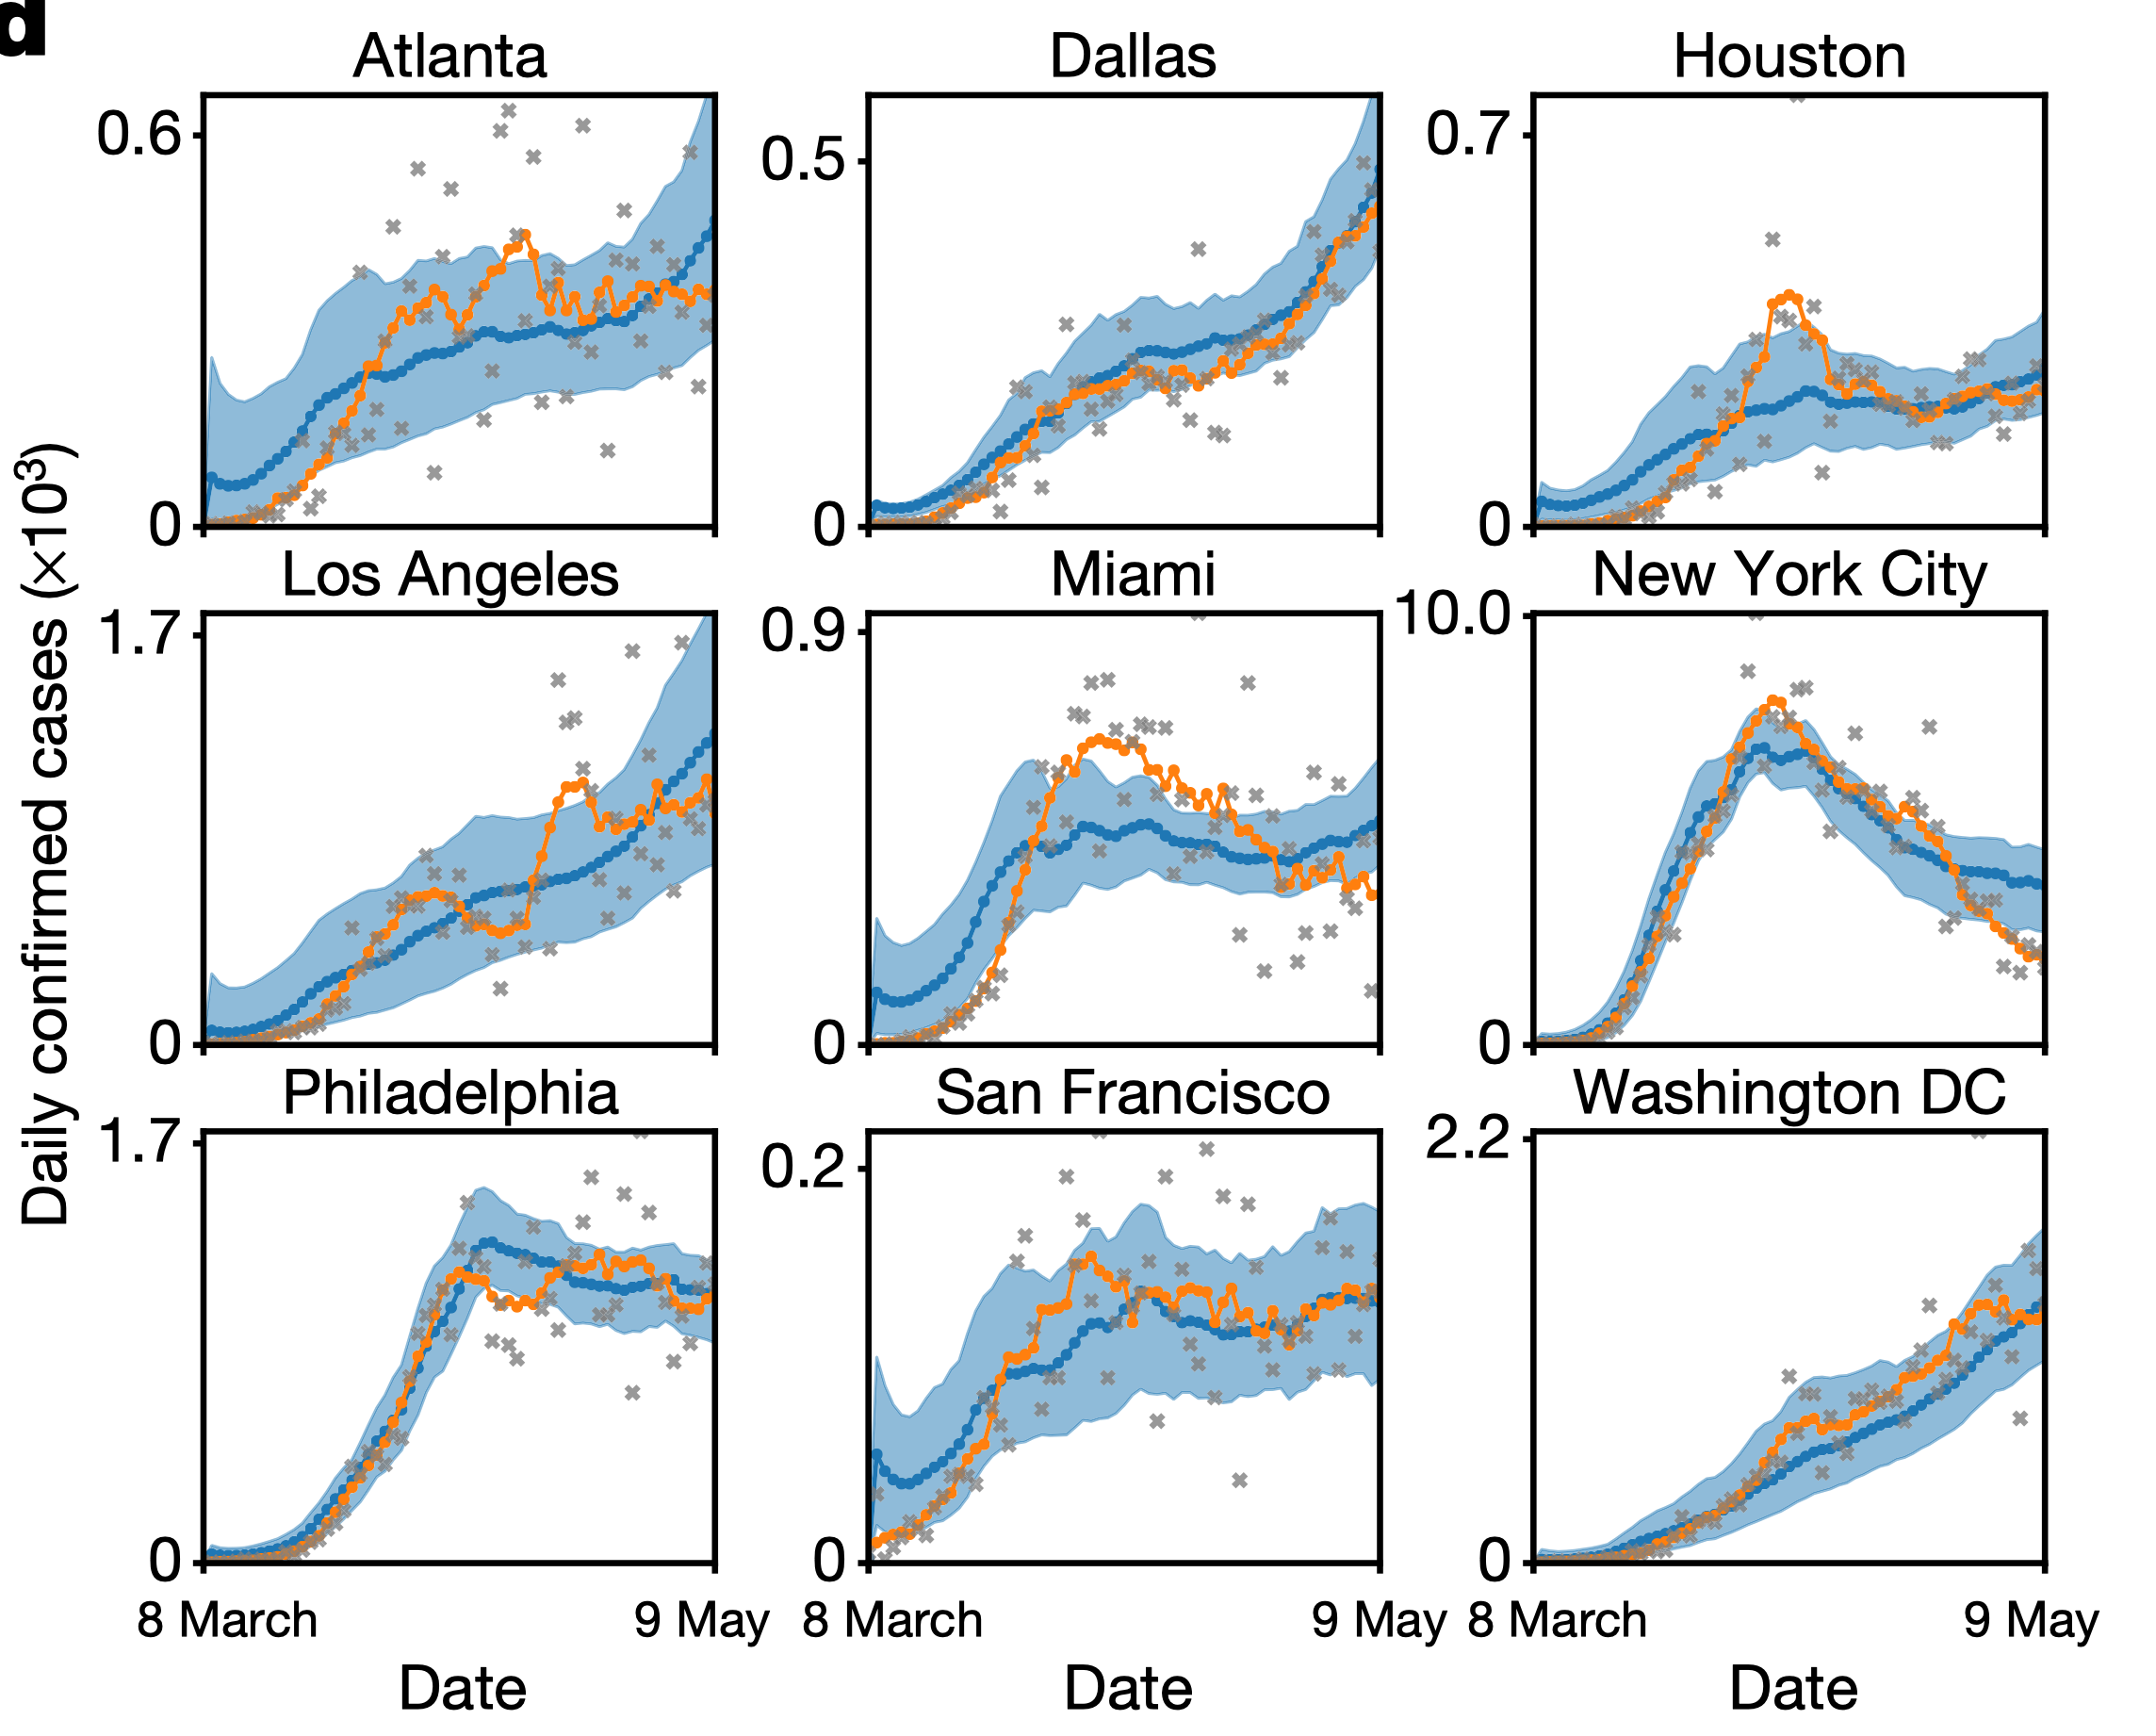
\includegraphics[width=\textwidth]{fig/prediction/predictions.png}
     \caption{各美國城市的預測結果}
     \label{fig:pred-cities}
\end{subfigure} 
\begin{subfigure}[b]{0.4\textwidth}
    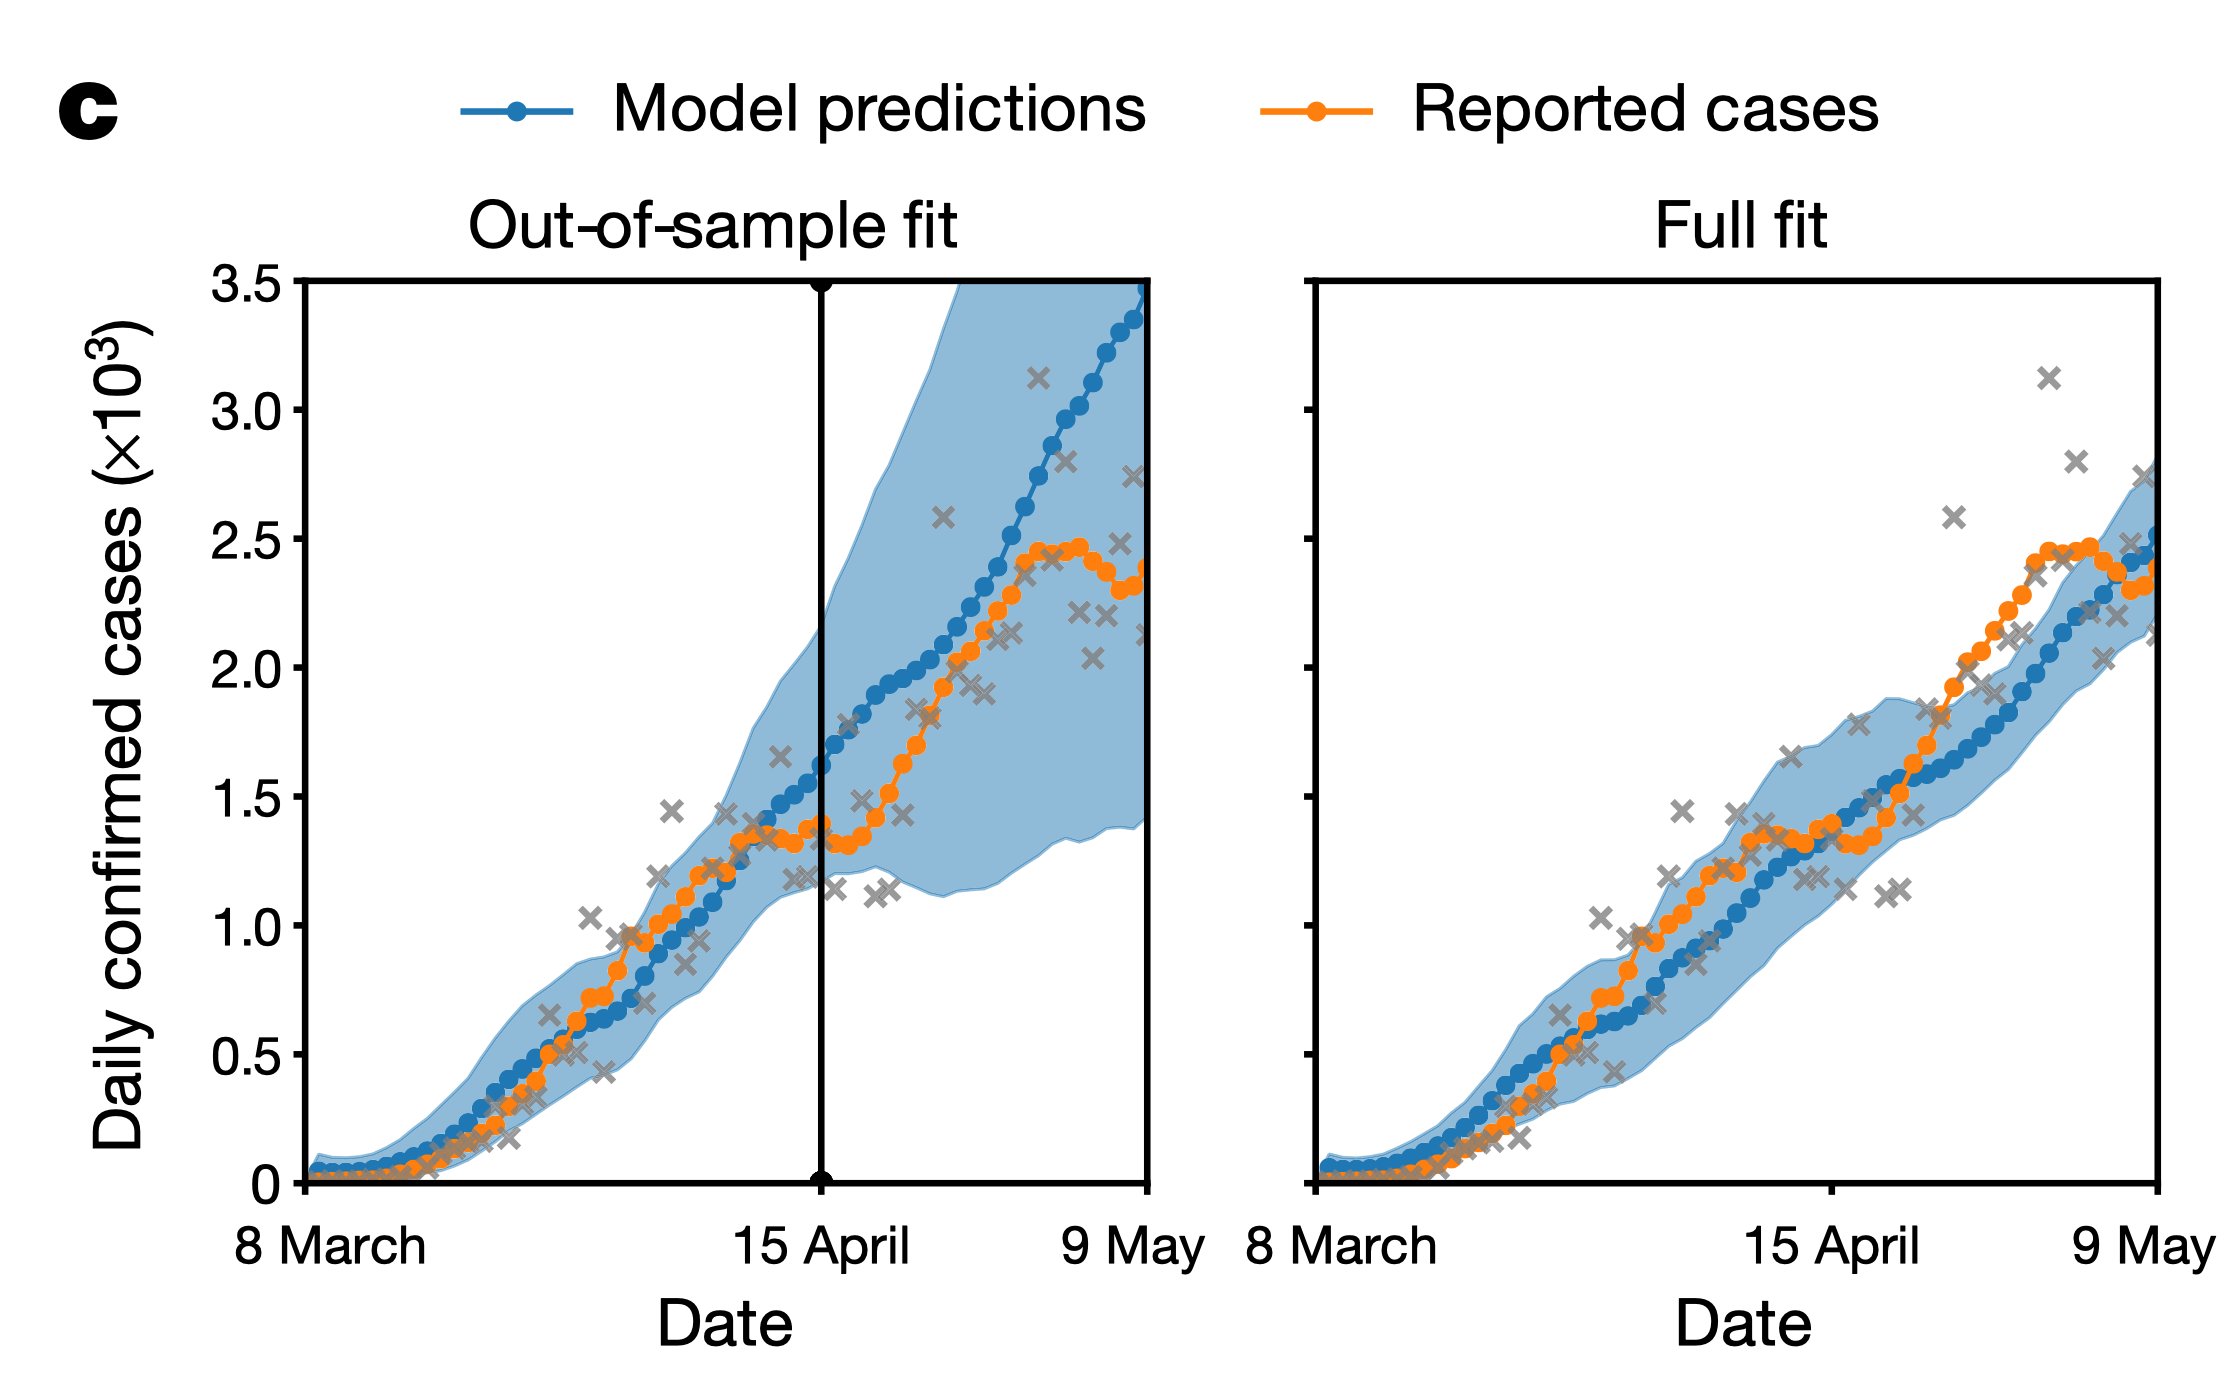
\includegraphics[width=\textwidth]{fig/prediction/compare.png}
    \caption{與簡化模型比較}
    \label{fig:pred-compare}
\end{subfigure}

\caption{\citeauthor{mobility2020} 的模擬結果。(a) 美國 9 座城市的每日新增感染人數對上時間圖。橘色線是真實的感染曲線,藍色線是預估的感染曲線。藍色區域則代表了 95$\%$信賴區間。 (b) compartment model 與單一模型比較。單一模型指的是將所有居住區域視為一個 SEIR 模型,不去計算區域之間的訪客,只有內部的交流。可以發現 compartment model (或稱為 coarse-grain model) 具有更好的預測。 左邊為單一簡單模型; 右邊為 compartment model (圖片節錄自 Fig. 1c/1d \cite{mobility2020}) }

\label{fig:pred}

\end{figure}